\section{Preliminary Results}
\begin{itemize}
    \item What examples can you handle already?
    \item What prototype have I built?
    \item How can I generalize these results? What problems have I identified or do I expect?
\end{itemize}

\begin{figure}[H]
  \centering

  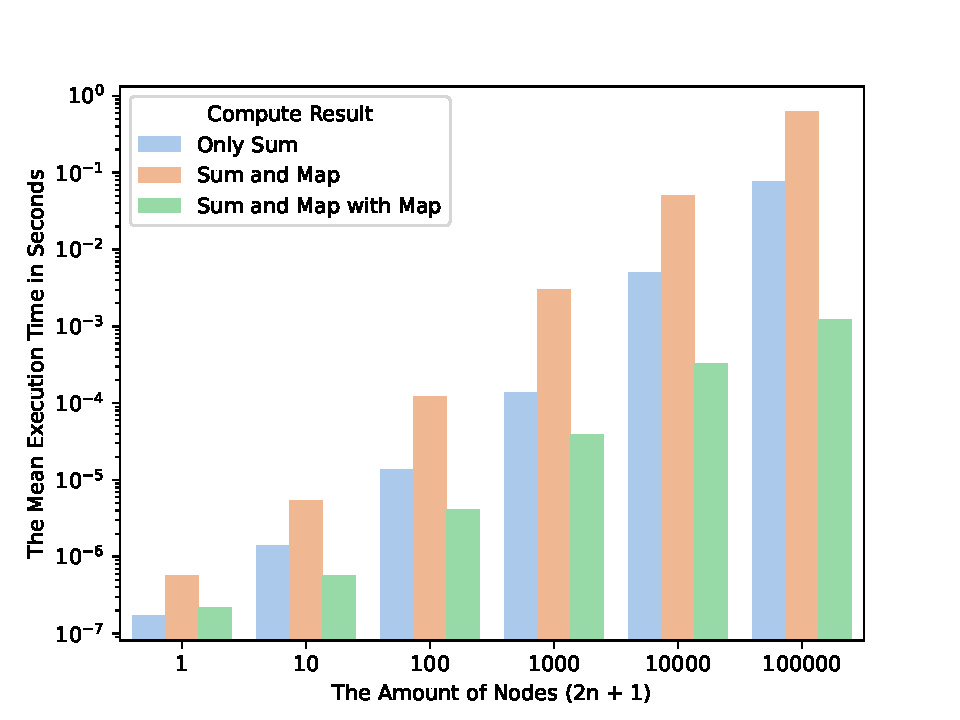
\includegraphics[width=.6\textwidth]{plot_generate_result_benchmark.pdf}
  \caption{Compute the result}
  \label{fig-compute-result}
\end{figure}


\begin{haskell}
merkle :: Merkelize f => Fix f -> Fix (f :*: K Digest)
merkle = In . merkleIn . unFix
\end{haskell}

\begin{haskell}
class (Functor f) => Merkelize f where
  merkleIn :: (Merkelize g) 
           => f (Fix g) -> (f :*: K Digest) (Fix (g :*: K Digest))
\end{haskell}

\begin{haskell}
data Tree a = Leaf a
            | Node (Tree a) a (Tree a)

type TreeG a = Fix (TreeF a)
type TreeF a = K a
            :+: ((I :*: K a) :*: I)
\end{haskell}

\begin{haskell}
cata :: Functor f => (f a -> a) -> Fix f -> a
cata alg t = alg (fmap (cata alg) (unFix t)) 
\end{haskell}

\begin{haskell}
cataSum :: TreeG Int -> Int
cataSum = cata (\case
  Inl (K x)                         -> x
  Inr (Pair (Pair (I l, K x), I r)) -> l + x + r)
\end{haskell}